\newpage
\section{Auswertung}
\label{sec:Auswertung}

\noindent
Alle Berechnungen werden mit Python mithilfe des Pakets \textsc{NumPy} \cite{numpy} durchgeführt und alle Plots mit \textsc{matplotlib} \cite{matplotlib} erstellt.
Die Fehlerrechnung erfolgt mit dem Paket \textsc{uncertainties} \cite{uncertainties}.

\subsection{Untersuchung des Spektrums}

\noindent
Das Spektrum der Caesium-Quelle mit Würfel 1 und Projektion I1 nach Abbildung \ref{fig:matrix} ist in Abbildung \ref{fig:spektrum} dargestellt. 
Zu erkennen ist die Anzahl der gemessenen Ereignisse in dem jeweiligen Channel, in dem sich die Ereignisse befinden.

\begin{figure}
  \centering
  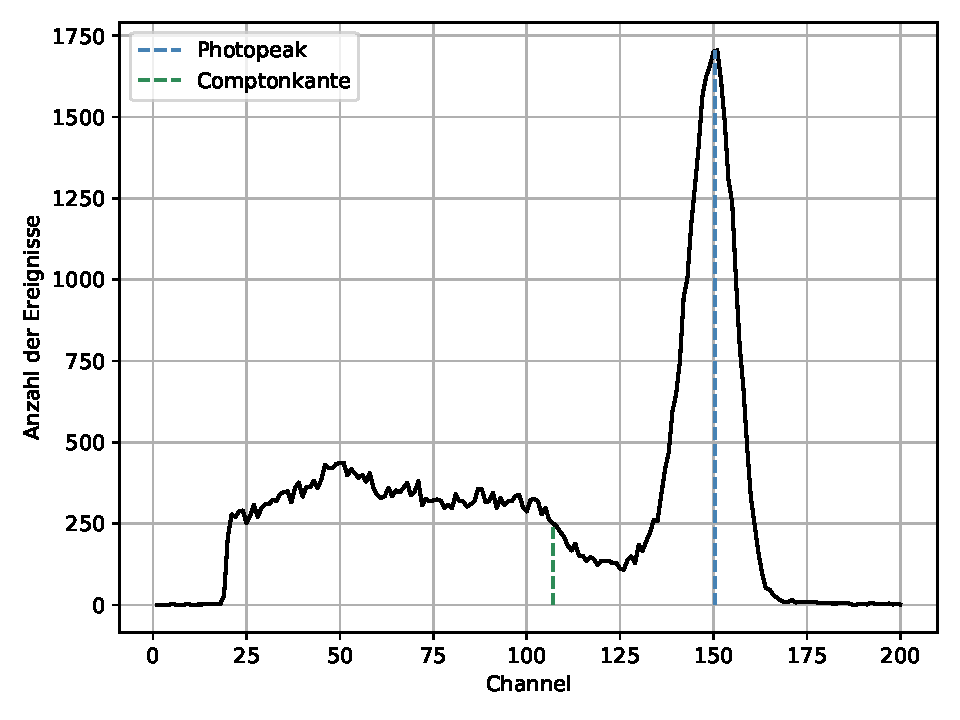
\includegraphics[width=\textwidth]{data/spektrum.pdf}
  \caption{Mit Würfel 1 und Projektion I1 aufgenoomenes Spektrum der Caesium-Quelle bei einer Messzeit von 150 Sekunden.}
  \label{fig:spektrum}
\end{figure}

\noindent
In dem Plot sind außerdem der Photopeak und die Comptonkante markiert.
Bei Caesium liegen die Energien dieser Größen bei $E_{P} = 662 \text{ keV}$ und $E_{C} = 478 \text{ keV}$ (Quelle:\cite{energien}).

\newpage
\subsection{Bestimmung der Absorptionskoeffizienten}
\noindent
Im folgenden wird die Nullmessung ausgewertet, wobei sich bei der Messung nur die Aluminiumhülle (Würfel 1) im Strahlengang befindet, die Teil jedes Würfels ist.
Die aufgenommenen Werte befinden sich in Tabelle \ref{tab:w1}.
Die Intensitäten $I$ werden durch

\begin{equation}
  I = \frac{N}{t}
\end{equation}

\noindent
bestimmt.

\begin{table}
  \centering
  \sisetup{table-format=2.1}
  \begin{tabular}{c c c c}
  \toprule
  $\text{Projektion}$ & $\text{Counts}$ & $\Delta t \,/\, s $ & $I_0 \,/\, \frac{1}{s} $\\
  \midrule 
    1  & 1705 & 150 & 11.37 $\pm$ 0.28 \\
    2  & 1440 & 135 & 10.67 $\pm$ 0.28 \\
    3  & 1571 & 142 & 11.06 $\pm$ 0.28 \\
    4  & 2111 & 166 & 12.72 $\pm$ 0.28 \\
    5  & 1424 & 102 & 13.72 $\pm$ 0.37 \\
    6  & 2444 & 180 & 13.58 $\pm$ 0.28 \\
    7  & 1633 & 165 & 9.90  $\pm$ 0.25 \\
    8  & 1554 & 115 & 13.51 $\pm$ 0.34 \\
    9  & 1126 & 107 & 10.52 $\pm$ 0.31 \\
    10 & 1434 & 110 & 13.04 $\pm$ 0.34 \\
    11 & 1432 & 102 & 14.04 $\pm$ 0.37 \\
    12 & 1036 &  76 & 13.63 $\pm$ 0.42 \\
  \bottomrule
  \end{tabular}
  \caption{Messwerte der $I_0$ Messung mit Würfel 1.}
  \label{tab:w1}
  \end{table}




\subsubsection{Würfel 2}

\noindent
Aus den Messdaten werden die Absorptionskoeffizienten $\mu_i$ nach 

\begin{equation}
\mu_i = \frac{\text{ln}(\frac{I_0}{I_i})}{d_i}
\label{eqn:mu}
\end{equation}

\noindent
bestimmt. Dabei ist $d_i$ die Strahlenlänge durch den Würfel je nach Projektion.
Es gilt:

\begin{align*}
d_{1,2,3,4,5,6} &= 3 \, \text{cm}       &\text{Senkrechte}\\
d_{7,9,10,12} &= 2 \sqrt{2} \, \text{cm} &\text{Nebendiagonale}\\
d_{8,11} &= 3 \sqrt{2} \, \text{cm} &\text{Hauptdiagonale}
\end{align*}

\begin{table}
  \centering
  \label{tab:w2}
  \sisetup{table-format=2.1}
  \begin{tabular}{c c c c c}
  \toprule
  $\text{Projektion}$ & $\text{Counts}$ & $\Delta t \,/\, s $ & $I_2 \,/\, \frac{1}{s} $ & $\mu \,/\, \frac{1}{cm}$\\
  \midrule 
 1 & 1770 & 180 & 9.83 $\pm$ 0.23  & 0.048   $\pm$ 0.011 \\
 2 & 1569 & 147 & 10.67 $\pm$ 0.27 & -0.0002 $\pm$ 0.012 \\
 3 & 1185 & 99 & 11.97 $\pm$ 0.35  & -0.026  $\pm$ 0.013 \\
 4 & 1731 & 150 & 11.54 $\pm$ 0.28  & 0.032   $\pm$ 0.011 \\
 5 & 1477 & 141 & 10.48 $\pm$ 0.27 & 0.095   $\pm$ 0.012 \\
 6 & 1417 & 123 & 11.52 $\pm$ 0.31  & 0.055   $\pm$ 0.011 \\
 7 & 1094 & 170 & 6.44 $\pm$ 0.20  & 0.152   $\pm$ 0.014 \\
 8 & 1580 & 150 & 10.53 $\pm$ 0.27 & 0.059   $\pm$  0.008\\
 9 & 1126 & 94 & 11.98 $\pm$ 0.36  & -0.045  $\pm$  0.015 \\
10 & 1337 & 160 & 8.36 $\pm$ 0.23  & 0.157   $\pm$ 0.013 \\
11 & 1805 & 199 & 9.07 $\pm$ 0.21   &  0.103  $\pm$ 0.008  \\
12 & 1063 & 147 & 7.23 $\pm$ 0.22  & 0.224   $\pm$ 0.015 \\
\bottomrule
\end{tabular}
\label{tab:w2}
\caption{Messwerte von Würfel 2.}
\end{table}

\noindent
Im folgenden werden die negativen Absorptionskoeffizienten nicht betrachtet, da diese nicht physikalisch sind.
Für Würfel 2 ergibt sich dann der gemittelte Absorptionskoeffizient $\mu_2 = 0.1029 \pm 0.0599 \, \frac{1}{cm}$.

  
  
\subsubsection{Würfel 3}

\noindent
Analog zu Würfel 2 werden auch hier die Absorptionskoeffizienten bestimmt.
Die dazugehörigen Daten befinden sich in Tabelle \ref{tab:w3}.

\begin{table}
\centering
\sisetup{table-format=2.1}
\begin{tabular}{c c c c c}
\toprule
$\text{Projektion}$ & $\text{Counts}$ & $\Delta t \,/\, s $ & $I_3 \,/\, \frac{1}{s} $ & $\mu \,/\, \frac{1}{cm} $\\
 \midrule 
 1 & 199  & 300 & 0.663 $\pm$ 0.047 & 0.947 $\pm$ 0.025  \\
 2 & 152  & 300 & 0.506 $\pm$ 0.041 & 1.016 $\pm$  0.028 \\
 3 & 165  & 300 & 0.55 $\pm$ 0.042  & 1.000 $\pm$ 0.027 \\
 10 & 156 & 300& 0.52 $\pm$  0.042  & 1.130 $\pm$  0.029\\
 11 & 95  & 300& 0.316 $\pm$ 0.032  & 0.892 $\pm$ 0.025 \\
 12 & 310 & 300& 1.033 $\pm$ 0.059  & 0.911 $\pm$ 0.021 \\
\bottomrule
\end{tabular}
\caption{Messwerte von Würfel 3.}
\label{tab:w3}
\end{table}

\noindent
Gemittelt ergibt sich für Würfel 3 $\mu_3 = 0.9827 \pm 0.011 \, \frac{1}{cm}$.

\subsubsection{Würfel 4}




    \noindent
    Da Würfel 4 aus verschiedenen kleinen Würfeln besteht, werden die Absorptionskoeffizienten mit dem gewichteten kleinste Quadrate fit nach
  
  \begin{equation}
  \vec{\mu} = ( A^\top W A)^{-1}(A^\top W \vec{I})
  \label{eqn:mu4}
  \end{equation}
  
  \noindent
  bestimmt, wobei die Unsicherheiten durch

  \begin{equation}
    V[\mu]= (A^{T}WA)^{-1}
    \label{eq7}
  \end{equation}

  \noindent
  gegeben sind.
  Die Elemente der diagonalen Gewichtsmatrix $W$ werden mithilfe der Gauß'schen Fehlerfortpflanzung nach
  
    \begin{align*}
        \sigma_{\text{j}}=& \left(\sqrt{\left(\frac{\sigma_{I_0}}{I_0}\right)^2+ \left(\frac{\sigma_{I_j}}{I_j}\right)^2}\right)\\
        W_{\text{jj}}=& \sigma_{\text{j}}^{-1}
    \end{align*}
    
    \noindent
    berechnet.

    \begin{table}
      \centering
      \sisetup{table-format=2.1}
      \begin{tabular}{c c c c c}
      \toprule
      $\text{Projektion}$ & $\text{Counts}$ & $\Delta t \,/\, s $ & $I_4 \,/\, \frac{1}{s} $ & $W_{jj}$\\
       \midrule 
    1  & 987  & 300 & 1.239  $\pm$ 0.039   & 25.002 \\
    2  & 1048 & 300 & 1.116 $\pm$ 0.041 &  24.628 \\
    3  & 1132 & 300 & 1.076 $\pm$ 0.039  & 25.65 \\
    4  & 1607 & 141 & 0.109 $\pm$ 0.033 &  30.206 \\
    5  & 212  & 300 & 2.983 $\pm$ 0.074  & 13.584 \\
    6  & 1917 & 169 & 0.179 $\pm$ 0.031 &  32.776 \\
    7  & 1558 & 300 & 0.645 $\pm$ 0.035  & 28.237 \\
    8  & 669  & 300 & 1.801  $\pm$ 0.046   &  21.625\\
    9  & 1248 & 300 & 0.928 $\pm$ 0.041  &  24.329\\
    10 &  2018 & 268 & 0.549 $\pm$  0.034 & 28.953  \\
    11 &  373  & 300 & 2.424 $\pm$ 0.058  & 17.202 \\
    12 &  1111 & 300 & 1.303 $\pm$ 0.043  & 23.153 \\
      \bottomrule
      \end{tabular}
      \caption{Messwerte von Würfel 4.}
      \label{tab:w4}
      \end{table}

\noindent
Daraus ergeben sich nach Gleichung \ref{eqn:mu4} folgende Absorptionskoeffizienten für Würfel 4 in Tabelle \ref{tab:muj}.

    \begin{table}
      \centering
      \sisetup{table-format=2.1}
      \begin{tabular}{c c}
      \toprule
      $\text{j}$ & $\mu_j \,/\, \frac{1}{cm}$ \\
       \midrule 
    1  & 0.182  $\pm$ 0.026\\
    2  & 0.606  $\pm$ 0.020\\
    3  & 0.366  $\pm$  0.026\\
    4  & -0.229 $\pm$ 0.019 \\
    5  & 1.278  $\pm$ 0.025 \\
    6  & -0.071 $\pm$ 0.020 \\
    7  & 0.143  $\pm$ 0.026 \\
    8  & 0.977  $\pm$ 0.022\\
    9  & -0.128 $\pm$  0.025 \\

      \bottomrule
      \end{tabular}
      \caption{Absorptionskoeffizienten von Würfel 4.}
      \label{tab:muj}
      \end{table}